% Options for packages loaded elsewhere
\PassOptionsToPackage{unicode}{hyperref}
\PassOptionsToPackage{hyphens}{url}
%
\documentclass[
]{article}
\usepackage{amsmath,amssymb}
\usepackage{lmodern}
\usepackage{iftex}
\ifPDFTeX
  \usepackage[T1]{fontenc}
  \usepackage[utf8]{inputenc}
  \usepackage{textcomp} % provide euro and other symbols
\else % if luatex or xetex
  \usepackage{unicode-math}
  \defaultfontfeatures{Scale=MatchLowercase}
  \defaultfontfeatures[\rmfamily]{Ligatures=TeX,Scale=1}
\fi
% Use upquote if available, for straight quotes in verbatim environments
\IfFileExists{upquote.sty}{\usepackage{upquote}}{}
\IfFileExists{microtype.sty}{% use microtype if available
  \usepackage[]{microtype}
  \UseMicrotypeSet[protrusion]{basicmath} % disable protrusion for tt fonts
}{}
\makeatletter
\@ifundefined{KOMAClassName}{% if non-KOMA class
  \IfFileExists{parskip.sty}{%
    \usepackage{parskip}
  }{% else
    \setlength{\parindent}{0pt}
    \setlength{\parskip}{6pt plus 2pt minus 1pt}}
}{% if KOMA class
  \KOMAoptions{parskip=half}}
\makeatother
\usepackage{xcolor}
\IfFileExists{xurl.sty}{\usepackage{xurl}}{} % add URL line breaks if available
\IfFileExists{bookmark.sty}{\usepackage{bookmark}}{\usepackage{hyperref}}
\hypersetup{
  hidelinks,
  pdftitle={A Timestep Crossover Law for Stochastically Rounded Velocity Verlet on a Harmonic Oscillator},
  pdfcreator={XeLaTeX}}
\urlstyle{same} % disable monospaced font for URLs
\usepackage[a4paper,margin=25mm]{geometry}
\usepackage{graphicx}
\makeatletter
\def\maxwidth{\ifdim\Gin@nat@width>\linewidth\linewidth\else\Gin@nat@width\fi}
\def\maxheight{\ifdim\Gin@nat@height>\textheight\textheight\else\Gin@nat@height\fi}
\makeatother
% Scale images if necessary, so that they will not overflow the page
% margins by default, and it is still possible to overwrite the defaults
% using explicit options in \includegraphics[width, height, ...]{}
\setkeys{Gin}{width=\maxwidth,height=\maxheight,keepaspectratio}
% Set default figure placement to htbp
\makeatletter
\def\fps@figure{htbp}
\makeatother
\setlength{\emergencystretch}{3em} % prevent overfull lines
\providecommand{\tightlist}{%
  \setlength{\itemsep}{0pt}\setlength{\parskip}{0pt}}
\setcounter{secnumdepth}{2}
\ifLuaTeX
  \usepackage{selnolig}  % disable illegal ligatures
\fi

\begin{document}

\begin{center}
\Large\bfseries A Timestep Crossover Law for Stochastically Rounded\\
Velocity Verlet on a Harmonic Oscillator
\\[0.75em]
\normalsize Cohen Brunner Thomas\\
\today
\end{center}

\begin{abstract}

We measure velocity-Verlet error for the unit harmonic oscillator,
separating ordinary FP32 round-to-nearest from stochastic rounding. In
the direct FP32 run, RMS final-state error has a grid minimum of
\(1.13\times10^{-5}\) at \(h=1.53\times10^{-3}\) and rises by factors
2.5 and 4.4 at the next two finer steps. For stochastic rounding, we use
the exact bias and variance decomposition and a common absolute timestep
grid across durations. The grid-minimum precision exponent is
\(\hat\beta_s=0.419\), with trajectory-bootstrap 95\% interval
[0.392, 0.448], which contains the predicted \(2/5\). An asymptotic
fixed-\(B\) prediction, calibrated from \(s=10,12,20,24\) without
\(s=16\), predicts the observed grid minima at five \(s=16\) duration
conditions to within 6.1\%. The duration exponent is
\(\hat\beta_T=-0.205\), with 95\% interval \([-0.254,-0.144]\),
which contains \(-1/5\). These results support the predicted scaling for
this oscillator and implementation.

\end{abstract}

\section{Introduction}\label{introduction}

For a fixed integration interval, reducing the step size decreases
Verlet's phase error but increases the number of floating-point updates.
The final-state error therefore reflects both the deterministic error of
the integrator and the accumulated effect of rounding. Its dependence on
step size also depends on the rounding rule.

Floating-point effects in symplectic integration have been studied by
Sanz-Serna and Calvo \cite{sanz1999} and are treated in the broader framework of
geometric numerical integration by Hairer, Lubich, and Wanner \cite{hairer2006}. For
stochastic rounding (SR), Connolly, Higham, and Mary prove
mean-independence results for rounding errors and use them to derive
probabilistic backward-error bounds for linear algebra \cite{connolly2021}. Kehlet and
Logg develop adjoint-weighted a posteriori ODE error estimates that
include roundoff. Under their error model, the accumulated roundoff term
scales inversely with the square root of the step size \cite{kehlet2017}. Croci et al.
survey SR analysis and applications, including ODE computation \cite{croci2022}.

Several studies examine probabilistic roundoff in ODE computation.
Mosbach and Turner model accumulated rounding errors in deterministic
ODE solvers and give trajectory distributions as functions of time, step
size, and precision \cite{mosbach2009}. Croci and Giles analyze round-to-nearest and SR
for Runge-Kutta finite-difference solutions of the heat equation and
derive bounds on rounding-error accumulation \cite{crocigiles2023}. Hopkins et al. study
SR in reduced-precision fixed-point solvers for neuron models, reporting
improved errors across several ODE solvers \cite{hopkins2020}.
Hairer, McLachlan, and Razakarivony show that implementation choices
affect long-time roundoff growth in Hamiltonian integration \cite{hairer2008}. Their
study concerns conservation errors for implicit Runge-Kutta schemes,
whereas our measured quantity is the final-state error of velocity
Verlet.

This paper tests a specific optimal-step law for velocity Verlet with
stochastic rounding on the unit harmonic oscillator. We calculate the
deterministic final-state bias from the exact Verlet matrix and estimate
the covariance trace from independent trajectories. Their sum gives the
mean-square risk without an independence assumption between truncation
and rounding errors. We derive an asymptotic law from the leading Verlet
phase term and a fitted covariance-growth model, then measure the
precision exponent and test a fixed-coefficient prediction across
duration. We fit the coefficient using significand widths 10, 12, 20,
and 24, then evaluate its predictions at width 16. The contribution is
this exact-bias and trajectory-covariance analysis with an absolute-scale
transfer test for one oscillator, integrator, rounding implementation,
and error metric. Its conclusions apply to that tested configuration.

We also report a separate FP32 round-to-nearest experiment. It shows a
crossover for this setup, while the stochastic-rounding experiment
isolates unbiased random rounding in a configurable binary format.

\section{System and methods}\label{system-and-methods}

We use the unit-frequency oscillator

\[
H(q,p)=\tfrac12(q^2+p^2),\qquad \dot q=p,\quad \dot p=-q,
\]

with the exact solution available analytically. We write the state as
\(x=(q,p)^\top\) and the exact state after time \(T\) as
\(x(T)=\Phi(T)x_0\), where \(\Phi(T)\) is the oscillator's rotation
matrix. The integration duration is \(T=100\) except in the duration
sweep. Kick-drift-kick velocity Verlet uses \(N\) equal steps of size
\(h=T/N\). The direct FP32/FP64 comparison uses 128 initial phases on
the unit-radius circle (energy \(H=1/2\)). The controlled stochastic-rounding sweep fixes
\(x_0=(1,0)^\top\) and uses 128 independent trajectories for the
precision sweep and 512 at each tested timestep in the duration sweep.

\subsection{Direct standard precision}\label{direct-standard-precision}

In the direct sweep, state values are rounded to IEEE FP32 or FP64 after
each Verlet stage. This tests accumulated state rounding in software and
does not emulate every hardware arithmetic pathway. For both precisions the sampled
step counts are \(N=2^k\), \(k=6,\ldots,18\).

\subsection{Stochastic rounding}\label{stochastic-rounding}

The controlled sweep uses binary significand widths
\(s\in\{8,10,12,16,20,24\}\). We use \(s\) for the number of
significand bits and reserve \(p\) for momentum. Exponents are
unbounded, isolating significand quantization. The coefficients \(h\) and
\(h/2\) are retained in FP64 to isolate rounding of the evolving state.
At \(T=100\), the precision sweep uses integer step counts obtained by
rounding \(2^{k/2}\), for \(k=12,13,\ldots,34\), and sets \(h=T/N\).
If an exact value \(z\) lies between adjacent representable numbers
\(z_-\le z\le z_+\), the operator returns

\[
\operatorname{SR}_s(z)=\begin{cases}
z_-,&\text{with probability }(z_+-z)/(z_+-z_-),\\
z_+,&\text{with probability }(z-z_-)/(z_+-z_-).
\end{cases}
\]

Thus \(\mathbb E[\operatorname{SR}_s(z)\mid z]=z\). Exactly
representable values remain unchanged. A seeded independent random
choice is made at each kick/drift state update (three rounding sites per
step). This is actual stochastic rounding of state updates, not additive
Gaussian noise. Arithmetic within each stage is evaluated before the
state value is rounded. We use unit-roundoff scale \(u=2^{-s}\) and
report ensemble RMS error over independent rounding trajectories.

The duration experiment holds \(s=16\) and uses the same widened
absolute grid \(h=1/k\) for every duration, with \(k=35,40,\ldots,200\).
Each duration is an integer, so \(N=Tk\) is integral and the grid is
identical across all five durations. The grid is fixed in advance rather
than centered on a theory-predicted optimum. The 170 duration/timestep
conditions use distinct, reproducibly seeded pseudorandom streams.

The implementation and raw results are
\href{experiment.py}{\texttt{experiment.py}},
\href{results/precision_sweep.csv}{\texttt{precision\_sweep.csv}},
\href{results/stochastic_sweep.csv}{\texttt{stochastic\_sweep.csv}}, and
\href{results/duration_sweep.csv}{\texttt{duration\_sweep.csv}}. Model
fits are saved in
\href{results/crossover_fit.json}{\texttt{crossover\_fit.json}} and
\href{results/duration_scaling.json}{\texttt{duration\_scaling.json}}.
The fixed-coefficient duration predictions are also available in
\href{results/fixed_b_duration_predictions.csv}{\texttt{fixed\_b\_duration\_predictions.csv}}.

\section{Quantitative crossover derivation}\label{quantitative-crossover-derivation}

For unit frequency, velocity Verlet is the linear map

\[
x_{n+1}=M_hx_n,\qquad M_h=\begin{pmatrix}1-h^2/2&h\\-h(1-h^2/4)&1-h^2/2\end{pmatrix}.
\]

The exact flow matrix is
\(\Phi(T)=\begin{pmatrix}\cos T&\sin T\\-\sin T&\cos T\end{pmatrix}\).
For the controlled sweep's initial state \(x_0=(1,0)^\top\), we take
binary64 as reference arithmetic and treat the stage operations as exact
relative to the simulated reduced precision. In this model, conditional
unbiasedness at each stochastic-rounding site gives
\(\mathbb E[X_N]=M_h^Nx_0\). Its bias relative to the exact solution is
\(b_h=M_h^Nx_0-\Phi(T)x_0\).

Within this reference-arithmetic model, the squared state error obeys
the bias and variance identity

\[
\mathcal J(h)=\mathbb E\|X_N-\Phi(T)x_0\|_2^2
=\|b_h\|_2^2+\operatorname{tr}(\Sigma_h),\qquad
\Sigma_h=\operatorname{Cov}(X_N).
\]

We compute the bias from the exact Verlet matrix and estimate the
covariance trace from replicate trajectories, so no independence
assumption between the two error sources is needed.
For errors \(e_j=X_N^{(j)}-\Phi(T)x_0\), \(j=1,\ldots,J\), the finite
ensemble identity is
\[
\frac1J\sum_{j=1}^J\|e_j\|_2^2
=\|\bar e\|_2^2+\frac1J\sum_{j=1}^J\|e_j-\bar e\|_2^2,
\qquad \bar e=\frac1J\sum_{j=1}^Je_j.
\]
Here \(J\) is the number of replicate trajectories. We estimate the
covariance with
\[
\widehat{\Sigma}_h=\frac{1}{J-1}\sum_{j=1}^J(e_j-\bar e)(e_j-\bar e)^\top,
\qquad
\widehat{\mathcal J}(h)=\|b_h\|_2^2+\operatorname{tr}(\widehat{\Sigma}_h).
\]
The coefficient \(B\) is fitted to the covariance term alone.

Write \(\theta_h=2\arcsin(h/2)\) and
\(\rho_h=\sqrt{1-h^2/4}\). The matrix power for \(x_0=(1,0)^\top\)
has the closed form

\[
M_h^Nx_0=(\cos(N\theta_h),-\rho_h\sin(N\theta_h))^\top.
\]

The modified angular frequency and amplitude factor satisfy

\[
\frac{\theta_h}{h}=1+\frac{h^2}{24}+O(h^4),
\qquad \rho_h=1-\frac{h^2}{8}+O(h^4).
\]

For fixed \(T\), the leading bias therefore contains both phase and
amplitude terms:

\[
b_h=h^2\begin{pmatrix}
-\frac{T}{24}\sin T\\[2pt]
-\frac{T}{24}\cos T+\frac18\sin T
\end{pmatrix}+O_T(h^4).
\]

Its exact leading coefficient is the norm of the displayed vector. For
large \(T\), this coefficient is \(T/24+O(1)\). We use the phase-only
coefficient \(A_{\mathrm{ph}}(T)=T/24\) for the simple asymptotic
prediction reported below. The full matrix bias enters every estimated
risk and grid minimum. Across the five tested durations, the exact
leading coefficient differs from \(A_{\mathrm{ph}}(T)\) by at most
1.6\%.

There are \(T/h\) steps. We model the measured trace covariance
asymptotically as

\[
E_{\mathrm{round}}(h)\simeq Bu\sqrt{T/h},
\]

where \(B\) absorbs the number and sensitivity of rounded updates per
step and details of this state metric. Substituting the phase-only bias
and covariance models into the bias and variance identity gives

\[
E_{\mathrm{rms}}^2(h)\simeq A_{\mathrm{ph}}(T)^2h^4+B^2u^2\frac{T}{h}.
\]

To estimate \(B\), we fit \(y_i\simeq B^2x_i\) by least squares through
the origin, where \(y_i\) is the unbiased trajectory-covariance trace
and \(x_i=u_i^2T/h_i\). The fit uses \(s=10,12,20,24\) at \(T=100\)
and \(h_i\leq0.2\). It excludes all \(s=16\) observations.

Differentiating with respect to \(h\) and setting the result to zero
yields

\[
\begin{aligned}
4A_{\mathrm{ph}}(T)^2h^3-B^2u^2T h^{-2}&=0,\\
h_{\star}&=\left(\frac{B^2u^2T}{4A_{\mathrm{ph}}(T)^2}\right)^{1/5}\\
&=\left(\frac{144B^2}{T}\right)^{1/5}u^{2/5}.
\end{aligned}
\]

The symbol \(h_\star\) denotes the continuous minimizer of this
asymptotic model. We use \(h_{\mathrm{grid}}\) for a minimum selected
from the tested timestep grid. Writing the predicted scaling as
\(h_\star\propto u^{\beta_s}T^{\beta_T}\) gives
\(\beta_s=2/5\) and \(\beta_T=-1/5\). The precision experiment
estimates \(B\). The duration sweep tests transfer of that estimate and
the predicted duration exponent.

\section{Results}\label{results}

\subsection{Direct FP32 crossover}\label{direct-fp32-crossover}

For FP32, the minimum sampled RMS final-state error is
\(1.13\times10^{-5}\) at \(h=1.5259\times10^{-3}\). At the next finer
step, \(h=7.6294\times10^{-4}\), error rises to \(2.80\times10^{-5}\).
at \(h=3.8147\times10^{-4}\) it is \(5.01\times10^{-5}\). Two successive
refinements therefore worsen this metric after the minimum. FP64
continues to improve through the finest tested step, reaching
\(6.06\times10^{-7}\), so its crossover is below or unresolved by this
grid (Figure~\ref{fig:direct}).

\begin{figure}[tbp]
\centering
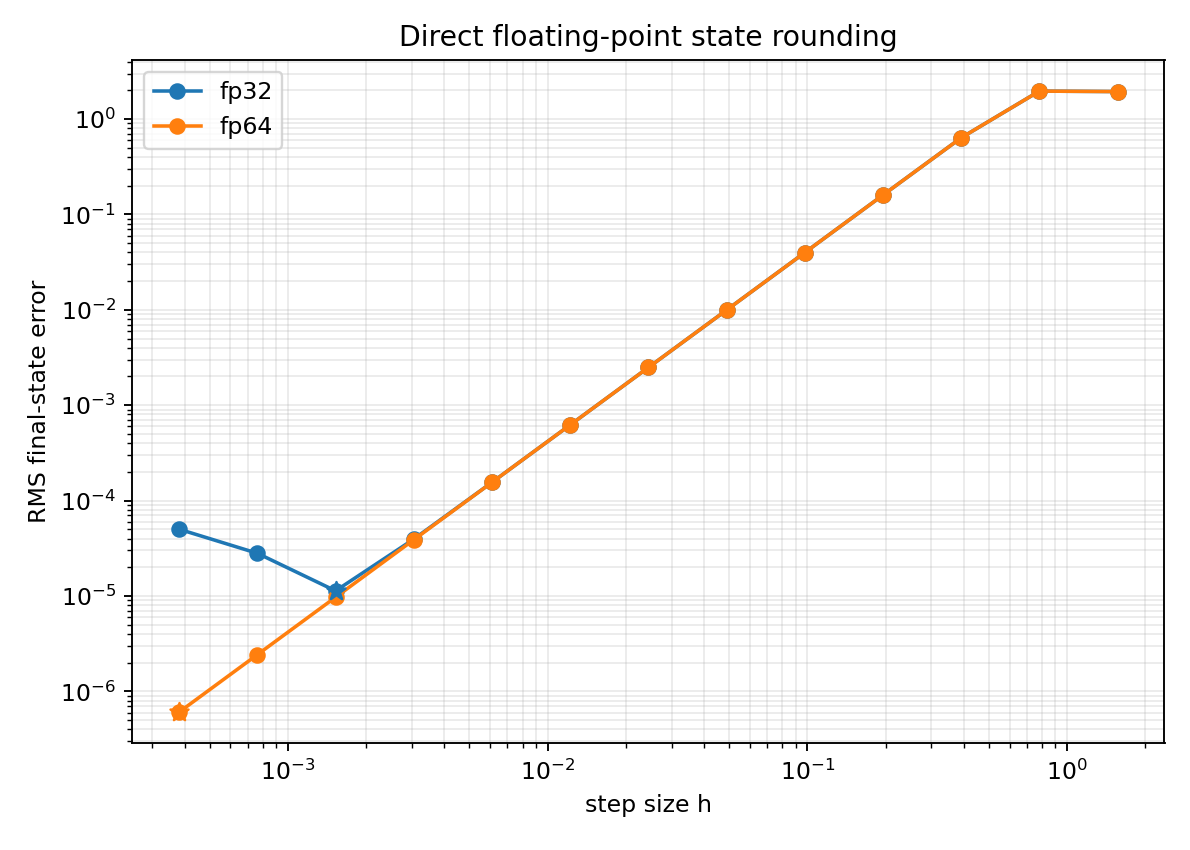
\includegraphics[width=0.82\textwidth]{results/precision_crossover.png}
\caption{Direct state rounding at \(T=100\), averaged over 128 initial
phases on the unit-radius circle. Stars mark grid minima.}
\label{fig:direct}
\end{figure}

\subsection{Stochastic-rounding crossover}\label{stochastic-rounding-crossover}

The grid-selected minimizing steps for \(s=10,12,16,20,24\) are
respectively \(4.883\times10^{-2}\), \(3.453\times10^{-2}\),
\(1.221\times10^{-2}\), \(2.158\times10^{-3}\), and
\(1.079\times10^{-3}\). For each width, let \(h_{\mathrm{grid}}\) be
the step that minimizes estimated risk on the tested grid. A least-squares
fit of \(\log h_{\mathrm{grid}}\) against \(\log u\), excluding \(s=8\),
gives \(\hat\beta_s=0.419\). We bootstrap
2,000 ensembles, resampling the 128 trajectories independently at every
precision and timestep, recomputing covariance risk, and reselecting each
minimum. The percentile 95\% interval for \(\hat\beta_s\) is
[0.392, 0.448], which includes the predicted exponent \(\beta_s=0.4\).
The per-width optimum intervals
are grid-selection intervals under this same bootstrap.
Fitting the exact matrix bias and measured covariance trace gives
\(B=0.6388\) using \(s=10,12,20,24\). Without refitting \(B\), the
asymptotic prediction at held-out \(s=16\) is \(h_\star=0.01065\),
versus the precision-sweep grid minimum \(h_{\mathrm{grid}}=0.01221\)
(12.8\% relative step error).

The \(s=8\) point is excluded from the primary exponent fit as the
coarsest simulated precision. Including it changes the slope only from
0.419 to 0.418. The minima are selected from a finite, half-octave step
grid, so the fitted slope is a resolution-limited estimate.
Figures~\ref{fig:sr-curves} and
\ref{fig:precision-scaling} show the error curves and the selected
optima.

\begin{figure}[tbp]
\centering
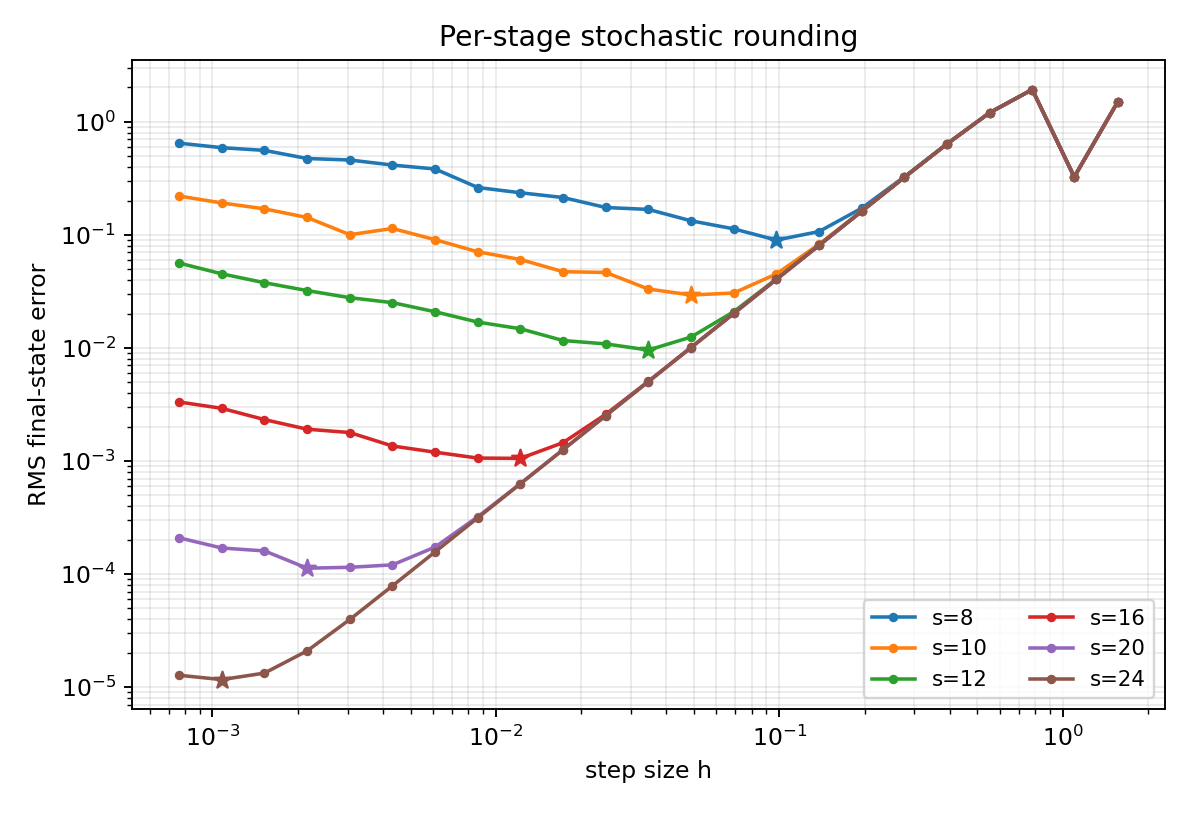
\includegraphics[width=0.82\textwidth]{results/stochastic_error_curves.png}
\caption{Estimated RMS final-state risk under stochastic rounding at
\(T=100\). Each curve uses the exact matrix bias and a sample covariance
trace from 128 trajectories per grid point. Stars mark grid minima.}
\label{fig:sr-curves}
\end{figure}

\begin{figure}[tbp]
\centering
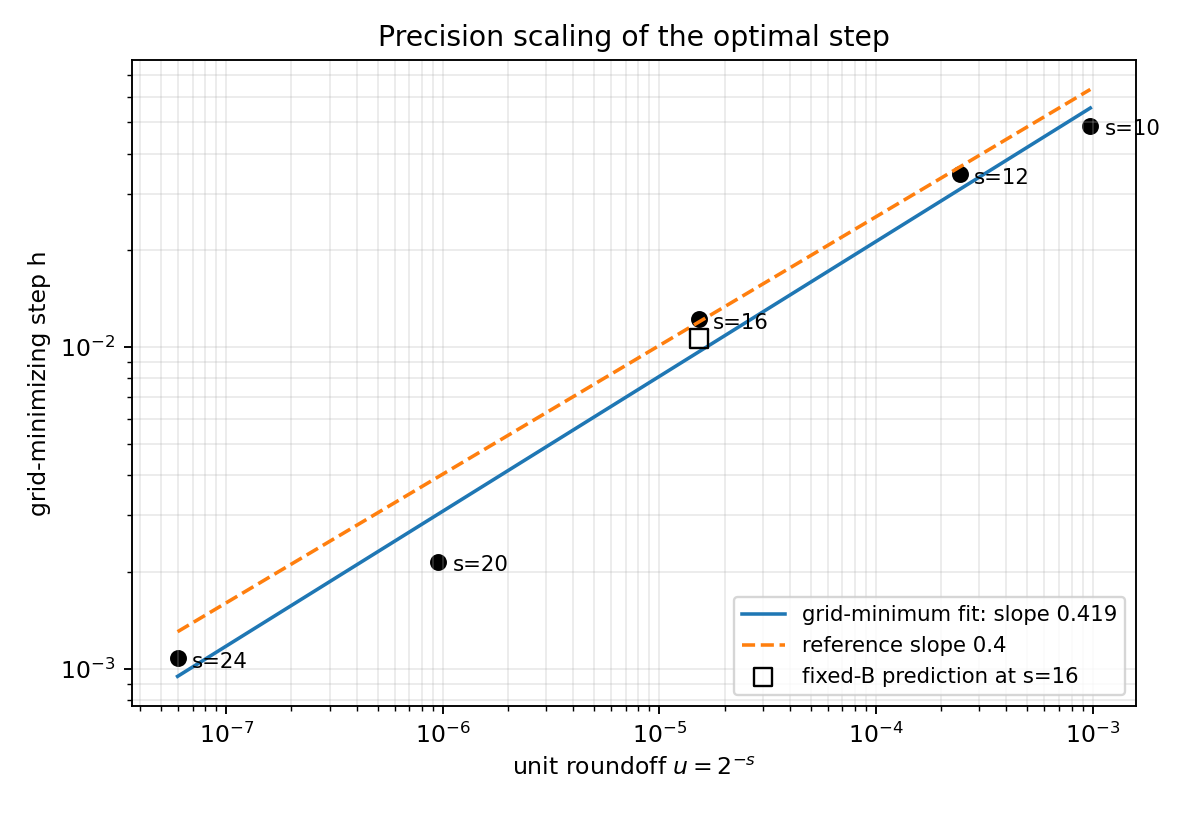
\includegraphics[width=0.82\textwidth]{results/precision_scaling.png}
\caption{Grid-minimizing steps versus unit-roundoff scale. The fitted
slope uses \(s=10,12,16,20,24\). The dashed reference line shares its
intercept with that fit. The open square is the asymptotic fixed-\(B\)
prediction calibrated without \(s=16\).}
\label{fig:precision-scaling}
\end{figure}

\subsection{Independent duration scaling}\label{independent-duration-scaling}

At held-out significand width \(s=16\), we test
\(T\in\{25,50,100,200,400\}\) with 512 independent rounding
trajectories per step on the common
widened grid. The bootstrap resamples the independently generated
trajectory ensemble separately at every timestep and duration, while
preserving paired state components within each trajectory. At each
bootstrap draw we re-estimate covariance and reselect each grid minimum.
Across 2,000 draws, the fitted exponent in
\(\log h_{\mathrm{grid}}\) versus \(\log T\) is
\(\hat\beta_T=-0.205\), with percentile 95\% interval
\([-0.254,-0.144]\). This interval contains the predicted
\(\beta_T=-0.2\). These intervals include trajectory-sampling and
grid-selection uncertainty conditional on the tested grids. They do not
include uncertainty in the separate fit of \(B\).

The asymptotic fixed-$B$ predictions below use \(B=0.6388\), fitted from the
\(T=100\) precision sweep at \(s=10,12,20,24\), and evaluate
\(h_\star(T)=(144B^2u^2/T)^{1/5}\) at \(u=2^{-16}\). Neither
the calibration nor these predictions use duration-sweep observations.
Observed minima are selected independently from the common grid.

\begin{table}[tbp]
\centering
\caption{Asymptotic fixed-\(B\) predictions and independently measured
duration-grid minima at \(s=16\). The interval is the percentile
trajectory-bootstrap interval for the selected grid minimum. Relative
difference is \((h_{\mathrm{grid}}-h_\star)/h_\star\).}
\label{tab:duration}
\begin{tabular}{rcccc}
\hline
Duration $T$ & Predicted $h_\star$ & Grid minimum $h_{\mathrm{grid}}$ & Bootstrap 95\% interval & Relative difference \\
\hline
25 & 0.01405 & 0.01333 & [0.01111, 0.01429] & $-5.1\%$ \\
50 & 0.01223 & 0.01250 & [0.01053, 0.01250] & $+2.2\%$ \\
100 & 0.01065 & 0.01000 & [0.00833, 0.01176] & $-6.1\%$ \\
200 & 0.00927 & 0.00909 & [0.00741, 0.01000] & $-1.9\%$ \\
400 & 0.00807 & 0.00769 & [0.00690, 0.00870] & $-4.7\%$ \\
\hline
\end{tabular}
\end{table}

This comparison tests calibration transfer in absolute scale across
duration, in addition to agreement of fitted exponents
(Table~\ref{tab:duration} and Figure~\ref{fig:duration}).

\begin{figure}[tbp]
\centering
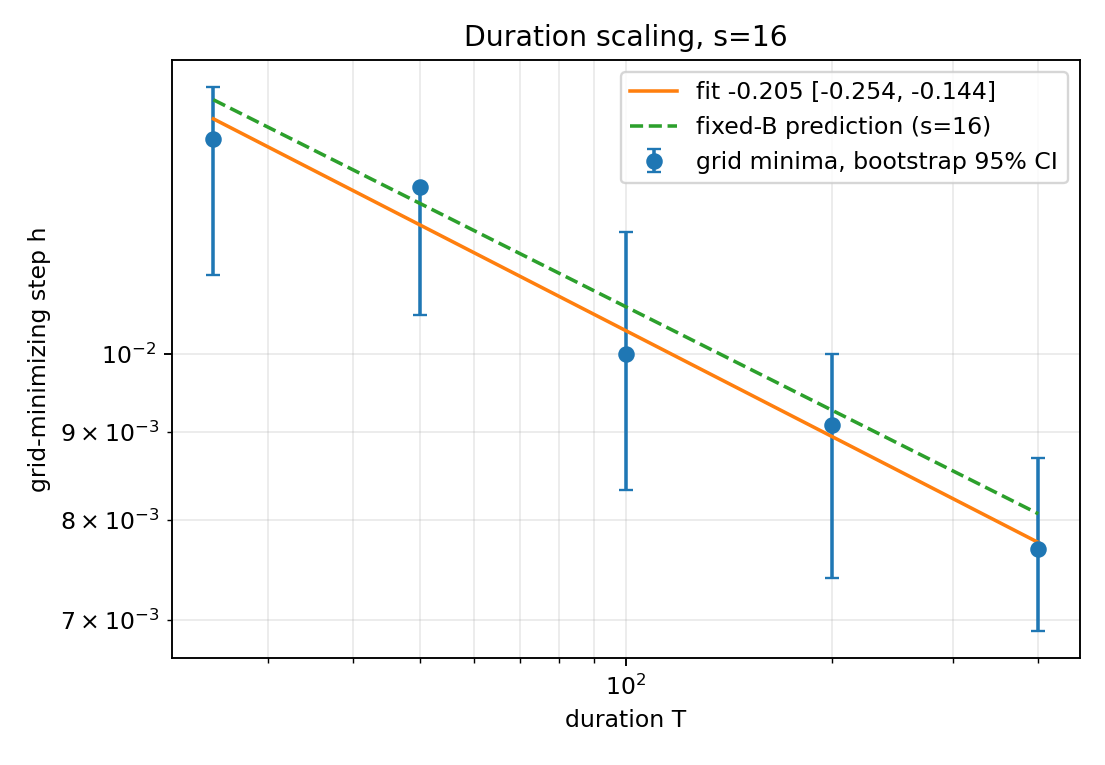
\includegraphics[width=0.82\textwidth]{results/duration_scaling.png}
\caption{Observed grid minima with 95\% trajectory-bootstrap intervals
and the asymptotic fixed-\(B\) prediction at \(s=16\). The same absolute
timestep grid is used at each duration.}
\label{fig:duration}
\end{figure}

\section{Discussion and limits}\label{discussion-and-limits}

The controlled experiment retains timestep coefficients in FP64 and
rounds only the three evolving state outputs per step. Its mean bias is
computed exactly from the Verlet matrix, while stochastic variance comes
from replicate covariance. The widened duration test uses one common
absolute \(h\) grid at all five durations. The \(s=16\) observations are excluded from
fitting \(B\) and held out for this test. Its point estimate and
bootstrap interval are compared with the prediction in the results. The
phase-only fixed-\(B\) curve predicts a continuous optimal step at each
duration. All five observed grid minima are within 6.1\% of the
predictions, and all five predictions lie inside the bootstrap intervals
for the observed minima. Separately, the fitted
fixed-\(B\) optimum is an out-of-sample precision check: it is 12.8\%
lower in step size than the observed \(s=16\) precision optimum.

The relation to previous roundoff studies is specific. Kehlet and Logg
estimate ODE solution error a posteriori by propagating local errors,
including roundoff, through an adjoint sensitivity calculation \cite{kehlet2017}.
Here, the deterministic bias is available in closed form, allowing us to
isolate stochastic covariance and test an explicit optimal-step
prediction. Connolly, Higham, and Mary analyze stochastic rounding
probabilistically and emphasize mean independence, which is weaker than
mutual independence \cite{connolly2021}. Fresh independent draws are used at each rounded
state update in our implementation, but recurrence propagation can
induce dependence in final-state errors. We measure the full trajectory
covariance instead of assuming that cross terms vanish. This is a
focused quantitative benchmark that complements these broader analyses.

The direct FP32 experiment and configurable stochastic-rounding
experiment answer different questions. The former uses standard
round-to-nearest and shows a clear crossover in this fixed oscillator.
The latter isolates unbiased random rounding and supports a fitted law.
Neither result alone proves that hardware roundoff behaves as
independent stochastic rounding, nor that the fitted \(B\) transfers to
other systems, integrators, durations, or observables. Real arithmetic
also has finite exponent ranges and operation-level rounding patterns
that this configurable format does not reproduce.

\section{Conclusion}\label{conclusion}

For \(T=100\), direct FP32 velocity Verlet has a state-error minimum
near \(h=1.5\times10^{-3}\) followed by increasing error under further
refinement. Under the specified simulated stochastic-rounding operator,
the exact
bias and variance decomposition and held-out common-grid duration sweep
give exponents \(\hat\beta_s=0.419\) versus \(u\) and
\(\hat\beta_T=-0.205\) versus \(T\). The modified-frequency expansion
and covariance-growth model give the long-duration phase approximation

\[
h_{\star}=\left(\frac{144B^2u^2}{T}\right)^{1/5}\propto u^{2/5}T^{-1/5}.
\]

The fit \(B=0.6388\), the precision exponent interval [0.392, 0.448],
its held-out \(s=16\) predictions, and duration-slope interval
\([-0.254,-0.144]\) quantify this controlled setup while keeping the
limits of the asymptotic model explicit.

\begin{thebibliography}{99}
\small
\bibitem{sanz1999}
  J. M. Sanz-Serna and M. P. Calvo, ``Symplectic integration with
  floating-point arithmetic and other approximations,'' \emph{Applied
  Numerical Mathematics}, 29(1), 3 to 18, 1999.
  \href{https://doi.org/10.1016/S0168-9274(98)00033-6}{doi:10.1016/S0168-9274(98)00033-6}.
\bibitem{hairer2006}
  E. Hairer, C. Lubich, and G. Wanner, \emph{Geometric Numerical
  Integration}, 2nd ed., Springer, 2006.
\bibitem{connolly2021}
  M. P. Connolly, N. J. Higham, and T. Mary, ``Stochastic Rounding and
  Its Probabilistic Backward Error Analysis,'' \emph{SIAM Journal on
  Scientific Computing}, 43(1), A566 to A585, 2021.
  \href{https://doi.org/10.1137/20M1334796}{doi:10.1137/20M1334796}.
\bibitem{kehlet2017}
  B. Kehlet and A. Logg, ``A posteriori error analysis of round-off
  errors in the numerical solution of ordinary differential equations,''
  \emph{Numerical Algorithms}, 76(1), 191 to 210, 2017.
  \href{https://doi.org/10.1007/s11075-016-0250-4}{doi:10.1007/s11075-016-0250-4}.
\bibitem{croci2022}
  M. Croci, M. Fasi, N. J. Higham, T. Mary, and M. Mikaitis, ``Stochastic
  rounding: implementation, error analysis and applications,'' \emph{Royal
  Society Open Science}, 9(3), 211631, 2022.
  \href{https://doi.org/10.1098/rsos.211631}{doi:10.1098/rsos.211631}.
\bibitem{mosbach2009}
  S. Mosbach and A. G. Turner, ``A quantitative probabilistic investigation
  into the accumulation of rounding errors in numerical ODE solution,''
  \emph{Computers and Mathematics with Applications}, 57(7), 1157 to 1167, 2009.
  \href{https://doi.org/10.1016/j.camwa.2009.01.020}{doi:10.1016/j.camwa.2009.01.020}.
\bibitem{crocigiles2023}
  M. Croci and M. B. Giles, ``Effects of round-to-nearest and stochastic
  rounding in the numerical solution of the heat equation in low precision,''
  \emph{IMA Journal of Numerical Analysis}, 43(3), 1358 to 1390, 2023.
  \href{https://doi.org/10.1093/imanum/drac012}{doi:10.1093/imanum/drac012}.
\bibitem{hopkins2020}
  M. Hopkins, M. Mikaitis, D. R. Lester, and S. Furber, ``Stochastic rounding
  and reduced-precision fixed-point arithmetic for solving neural ordinary
  differential equations,'' \emph{Philosophical Transactions of the Royal
  Society A}, 378(2166), 20190052, 2020.
  \href{https://doi.org/10.1098/rsta.2019.0052}{doi:10.1098/rsta.2019.0052}.
\bibitem{hairer2008}
  E. Hairer, R. I. McLachlan, and A. Razakarivony, ``Achieving Brouwer's
  law with implicit Runge-Kutta methods,'' \emph{BIT Numerical
  Mathematics}, 48(2), 231 to 243, 2008.
  \href{https://doi.org/10.1007/s10543-008-0170-3}{doi:10.1007/s10543-008-0170-3}.
\end{thebibliography}

\end{document}
